\documentclass{article}
\usepackage{amsmath}
\usepackage{amssymb}
\usepackage{booktabs}
\usepackage{xintexpr}
\usepackage{subcaption}
\usepackage{float}
\usepackage{enumitem}
\usepackage{tikz}
\usetikzlibrary{arrows,automata}

\newcommand{\T}{1}
\newcommand{\F}{0}
\newcommand{\TF}[1]{\if1#1\T\else\F\fi}
\newcommand{\xintTF}[1]{\xintifboolexpr{#1}{\T}{\F}}

\newcommand{\logicrule}[2]{
\begin{array}{l}
#1 \\
\midrule
\therefore #2 \\
\end{array}
}

\newcommand{\inv}[1]{#1^{-1}}

\renewcommand{\d}[1]{\,\textnormal{d}#1}
\newcommand{\dd}[2]{\frac{\d{#1}}{\d{#2}}}
\newcommand{\ddd}[2]{\dfrac{\d{#1}}{\d{#2}}}

\DeclareMathOperator{\var}{Var}
\DeclareMathOperator{\E}{\mathcal{E}}

\newcommand{\multistep}[1]{\begin{array}{rl} #1 \end{array}}
\newcommand{\subeq}{\subseteq}
\newcommand{\sub}{\subset}

\newcommand{\conj}[1]{\overline{#1}}

\setlength\parindent{0pt}
\setlength\parskip{1em}

\begin{document}

\section*{New Computation Model}

\textbf{Pushdown Automata (PDA)}: like an NFA but has a
\textbf{stack}.

\begin{itemize}
\item Stack provides additional memory beyond the finite memory
  available in ``cmsol''.
\item Stack allows PDA to recognize some \textbf{non-regular}
  languages.
\end{itemize}

There are 2 options to prove a language is context-free:

\begin{enumerate}
\item Construct a CFG that \textbf{generates} it
\item Construct a PDA that \textbf{recognizes} it.
\end{enumerate}

\subsection*{Schematic}

\begin{figure}[H]
  \centering
  \begin{subfigure}{.5\textwidth}
    \centering
    $\boxed{Finite Control}\rightarrow\boxed{a|a|b|b}$
    \caption{NFA}
  \end{subfigure}%
  %
  \begin{subfigure}{.5\textwidth}
    \centering
    Finite control $\rightarrow$ Input and Stack
    \caption{PDA}
  \end{subfigure}
\end{figure}

\subsection*{Terminology}

\begin{description}
\item[Push]: Write a symbol on stack
\item[Pop]: Remove a symbol from stack
\item[Stack]: LIFO storage device
\end{description}

\subsection*{Benefits}

\begin{itemize}
\item Can hold \textbf{unlimited} amount of info
\item PDA can recognize $\{0^n1^n|n\ge0\}$ because it can use the
  stack to \textbf{remember} the number of $0$'s it has seen.
\end{itemize}

\subsection*{Informal Algorithm}

Recognize $\{0^n1^n|n\ge0\}$.

\begin{enumerate}
\item Read symbol from input. As each $0$ is ead, push it onto the
  stack.
\item As soon as a $1$ is read, pop a $0$ off the stack for each $1$
  read.
\item If input finishes when stack becomes empty, \textbf{accept}. If
  stack becomes empty while there is still input or inpt ends while
  stack is not empty, \textbf{reject}.
\end{enumerate}

\subsection*{Nature of PDA}

\begin{itemize}
\item PDA may be \textbf{nondeterministic}. $\{0^n1^n|n\ge0\}$ does
  not require nondeterminism. $\{ww^R|w\in\{0,1\}^*\}$ does require
  nondeterminism.
\end{itemize}

\subsection*{PDA}

\begin{itemize}
\item May use different alphabet for input ($\Sigma$) and stack
  ($\Gamma$).
\item Nondeterminism allows PDA to make transitions on empty input.

  \[
  \Sigma_\epsilon = \Sigma\cup\{\epsilon\}
  \] \[
  \Gamma_\epsilon = \Gamma\cup\{\epsilon\}
  \]

  Domain of PDA transition function is
  $Q\times\Sigma_\epsilon\times\Gamma_\epsilon$.

  Range of PDA transition functon is $2^{Q\times\Gamma_\epsilon}$.

  \[
  \delta:Q\times\Sigma_\epsilon\times\Gamma_\epsilon\rightarrow2^{Q\times\Gamma_\epsilon}
  \]
\end{itemize}

\subsection*{Formal Definition}

Given as a 6-tuple: $(Q,\Sigma,\Gamma,\delta,q_0,F)$.

\begin{description}
\item[$Q$]: set of states
\item[$\Sigma$]: alphabet (input)
\item[$\Gamma$]: alphabet (stack)
\item[$\delta$]: $Q\times\Sigma_\epsilon\times\Gamma_\epsilon\rightarrow2^{Q\times\Gamma_\epsilon}$
\item[$q_0\in{}Q$]: start state
\item[$F\subseteq{}Q$]: accept states
\end{description}

\subsection*{PDA Computation}

A PDA $M=(Q,\Sigma,\Gamma,\delta,q_0,F)$ computes as follows:

\begin{itemize}
\item $m$ inputs $w=w_1w_2\cdots,w_m\in\Sigma_\epsilon$
\item Sequence of states $r_0,r_1,\cdots,r_m\in{}Q$
\item Sequence of strings $s_0,s_1,\cdots,s_n\in\Gamma^*$
\item Accepted if we statisfy the following conditions:
  \begin{enumerate}[label=(\arabic*)]
    \item $r_0=q_0$, $s_0=\epsilon$ ($M$ begins with start state and
      empty state)

    \item For $i=0,1,\cdots,m_1$ we have
      $(r_{i+1},b)\in\delta(r_i,w_{i+1},a)$ where $s_i=at$ and
      $s_{i+1}=bt$ for some $a,b\in\Gamma$ and $t\in\Gamma^*$. ($M$
      moves according to state, stack input symbol)

    \item $r_m\in{}F$ (has to reach an accept state)
  \end{enumerate}
\end{itemize}

\subsection*{Example: PDA}

For the language $L=\{0^n1^n|n\ge0\}$.

\[
M_1=(Q,\Sigma,\Gamma,\delta,q_1,F)
\]

Where

\begin{description}
\item[$Q$]$=\{q_1,q_2,q_3,q_4\}$
\item[$\Sigma$]$=\{0,1\}$
\item[$\Gamma$]$=\{0,\$\}$
\item[$F$]$=\{q_1,q_4\}$
\end{description}

$\delta$ is given as:

\[\begin{array}{c|ccc|ccc|ccc}
\Sigma_\epsilon & & 0 &  & 1 &  & \epsilon & \\
\Gamma_\epsilon & 0 & \$ & \epsilon & 0 & \$ & \epsilon & 0 & \$ & \epsilon \\
\midrule
q_1 & \\
q_2 &   &   &     & (q_3,\epsilon) \\
q_3 &   &   &  (q_2,0) \\
q_4 & \\
\end{array}\]

\begin{figure}[H]
  \centering
  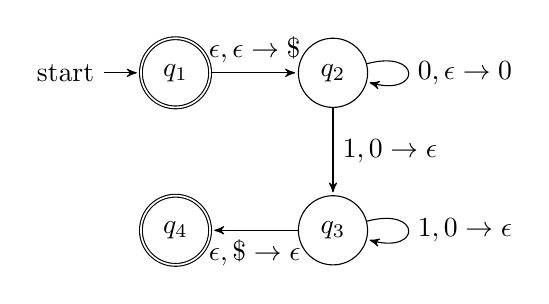
\begin{tikzpicture}[>=stealth',shorten >=1pt,auto,node distance=2cm]
    \node[initial,state,accepting] (q1) {$q_1$};
    \node[state] (q2) [right of=q1] {$q_2$};
    \node[state] (q3) [below of=q2] {$q_3$};
    \node[state,accepting] (q4) [below of=q1] {$q_4$};

    \path[->]
    (q1) edge node {$\epsilon,\epsilon\rightarrow\$$} (q2)

    (q2) edge [loop right] node {$0,\epsilon\rightarrow0$} (q2)
    (q2) edge node {$1,0\rightarrow\epsilon$} (q3)

    (q3) edge [loop right] node {$1,0\rightarrow\epsilon$} (q3)
    (q3) edge node {$\epsilon,\$\rightarrow\epsilon$} (q4)
    ;
  \end{tikzpicture}
  \caption{$M_1$}
\end{figure}

\subsection*{Stack Interpretation}

\[
a,b\rightarrow c
\]

\begin{description}
\item[$a$]: read input
\item[$b$]: pop from stack
\item[$c$]: push onto stack
\end{description}

If $a=\epsilon$, machine \textbf{can} transition without reading any
input.

If $b=\epsilon$, machine \textbf{can} transition with \textbf{reading}
and \textbf{popping} any symbol from stack.

If $c=\epsilon$, machine \textbf{can} transition without writing any
symbol onto stack.

\subsection*{Notes}

The PDA definition does \textbf{not consider} test of \textbf{empty
  stack}. (place $\$$ on stack to read).

\subsection*{Example 2}

$M_2$ should recognize $\{a^ib^jc^k|i,j,k\ge0\wedge{}i=j\vee{}i=k\}$.

\end{document}
